\documentclass[../master/master.tex]{subfiles}

\begin{document}

%----------------------------------------------------------------------
% LECTURE 3: Set Theory
% Date: January 27, 2026
%----------------------------------------------------------------------
\renewcommand{\lecturenum}{3}
\renewcommand{\lecturedate}{January 27, 2026}
\renewcommand{\lecturetopic}{Set Theory}

\section{Lecture \lecturenum : \lecturedate}

\begin{lecturesummary}
\textbf{Lecture Overview:} We develop the set-theoretic foundations needed for analysis. We define \textbf{functions} as special relations and introduce key properties: surjectivity, injectivity, and bijectivity. Using bijections, we define when two sets have the same \textbf{cardinality}, leading to the notions of \textbf{finite}, \textbf{infinite}, and \textbf{countable} sets.
\end{lecturesummary}

\subsection{Functions}

\begin{summarybox}
\textbf{Section Overview:} We define functions as relations with a uniqueness property, introduce images and preimages, and classify functions as injective (one-to-one), surjective (onto), or bijective (both).
\end{summarybox}

\begin{definition}
A \defn{function} $f: A \to B$ is a relation $R \subseteq A \times B$ such that for all $x \in A$, there exists a unique $y \in B$ with $(x, y) \in R$. This $y$ is denoted $f(x)$. The set $A$ is called the \defn{domain} of $f$, and $B$ is the \defn{codomain} (or \defn{range}).
\end{definition}

\begin{remark}
Not all relations are functions. A relation fails to be a function if some element of $A$ maps to multiple elements of $B$, or to no element at all.
\end{remark}

\begin{definition}
Let $f: A \to B$ be a function.
\begin{itemize}
    \item If $E \subseteq A$, the \defn{image} of $E$ under $f$ is $f(E) = \{f(x) : x \in E\}$.
    \item If $F \subseteq B$, the \defn{preimage} of $F$ under $f$ is $f^{-1}(F) = \{x \in A : f(x) \in F\}$.
\end{itemize}
\end{definition}

\begin{definition}
Let $f: A \to B$ be a function.
\begin{itemize}
    \item $f$ is \defn{surjective} (or \defn{onto}) if $f(A) = B$, i.e., for every $y \in B$, there exists $x \in A$ with $f(x) = y$.
    \item $f$ is \defn{injective} (or \defn{one-to-one}) if $f(x_1) = f(x_2)$ implies $x_1 = x_2$, i.e., distinct inputs map to distinct outputs.
    \item $f$ is \defn{bijective} if it is both injective and surjective.
\end{itemize}
\end{definition}

\subsection{Equivalence Relations}

\begin{summarybox}
\textbf{Section Overview:} We review equivalence relations and observe how function properties relate to composition and inverses.
\end{summarybox}

\begin{remark}
Recall from Lecture 1 that an equivalence relation satisfies:
\begin{itemize}
    \item \textbf{Reflexivity:} $x \sim x$ (like the identity function)
    \item \textbf{Symmetry:} $x \sim y \Rightarrow y \sim x$ (like invertible functions: if $f: A \to B$, then $f^{-1}: B \to A$)
    \item \textbf{Transitivity:} $x \sim y$ and $y \sim z \Rightarrow x \sim z$ (like composition: $f: A \to B$ and $g: B \to C$ give $g \circ f: A \to C$)
\end{itemize}
\end{remark}

\subsection{Cardinality}

\begin{summarybox}
\textbf{Section Overview:} We define cardinality using bijections, then classify sets as finite, infinite, or countable.
\end{summarybox}

\begin{definition}
Two sets $A$ and $B$ have the same \defn{cardinality}, written $A \sim B$, if there exists a bijection $f: A \to B$.
\end{definition}

\begin{definition}
Let $[n] = \{1, 2, 3, \ldots, n\}$. We say that a set $A$ is:
\begin{enumerate}
    \item \defn{finite} if there exists $n \in \N$ such that $A \sim [n]$,
    \item \defn{infinite} if $A$ is not finite,
    \item \defn{countable} if $A \sim \N$.
\end{enumerate}
\end{definition}

\begin{example}
$\Z$ is countable. We can list the integers as:
\[
0, 1, -1, 2, -2, 3, -3, \ldots
\]
This defines a bijection $f: \N \to \Z$ given by
\[
f(n) = \begin{cases}
-\frac{n}{2} & \text{if } n \text{ is even} \\[4pt]
\frac{n+1}{2} & \text{if } n \text{ is odd}
\end{cases}
\]
(where we start $\N$ at $0$). Thus $\Z \sim \N$, so $\Z$ is countable.
\end{example}

\begin{definition}
A \defn{sequence} is a function $f: \N \to X$ where $X$ is some set. If we denote $f(n)$ by $x_n$, then we write the sequence as $(x_n)_{n=1}^{\infty}$.
\end{definition}

\begin{remark}
If $A$ is a countable set, then there exists a surjection $f: \N \to A$. We say that $A$ can be \defn{arranged in a sequence}: the elements of $A$ can be listed as $f(1), f(2), f(3), \ldots$
\end{remark}

\begin{notebox}
\textbf{Note:} The \defn{set difference} $A \setminus B$ (read ``$A$ minus $B$'') is defined as
\[
A \setminus B = \{x \in A : x \notin B\}.
\]
\end{notebox}

\begin{theorem}
Every infinite subset of a countable set is countable.
\end{theorem}

\begin{proof}
Let $A$ be a countable set and let $B \subseteq A$ be infinite. Since $A$ is countable, we can arrange its elements as a sequence $(x_n)_{n=1}^{\infty}$.

We construct a bijection $f: \N \to B$ inductively. Let $B_0 = \emptyset$. For each $k \geq 1$:
\begin{itemize}
    \item Let $n_k = \min\{n \in \N : x_n \in B \setminus B_{k-1}\}$
    \item Define $f(k) = x_{n_k}$
    \item Set $B_k = B_{k-1} \cup \{x_{n_k}\}$
\end{itemize}
At each step, $x_{n_k}$ is assigned position $k = |B_{k-1}| + 1$ in our enumeration of $B$. Since $B$ is infinite, we never exhaust it, so each $n_k$ exists.

This $f$ is a bijection: it is injective since each element is added exactly once, and surjective since every element of $B$ appears at some position $n$ in the sequence $(x_n)$ and will eventually be enumerated.

Thus $B \sim \N$, so $B$ is countable.
\end{proof}

\subsection{Unions and Intersections of Sets}

\begin{summarybox}
\textbf{Section Overview:} We define unions and intersections of collections of sets, including arbitrary (possibly infinite) unions and intersections.
\end{summarybox}

\begin{center}
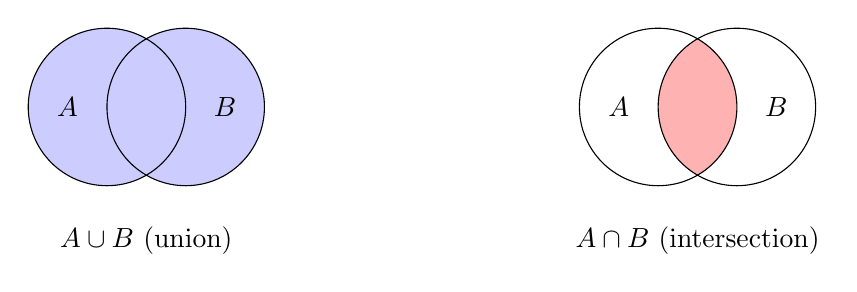
\begin{tikzpicture}
    % Union
    \begin{scope}[shift={(-3.5,0)}]
        \fill[blue!20] (0,0) circle (1);
        \fill[blue!20] (1,0) circle (1);
        \draw (0,0) circle (1);
        \draw (1,0) circle (1);
        \node at (-0.5,0) {$A$};
        \node at (1.5,0) {$B$};
        \node at (0.5,-1.7) {$A \cup B$ (union)};
    \end{scope}

    % Intersection
    \begin{scope}[shift={(3.5,0)}]
        \begin{scope}
            \clip (0,0) circle (1);
            \fill[red!30] (1,0) circle (1);
        \end{scope}
        \draw (0,0) circle (1);
        \draw (1,0) circle (1);
        \node at (-0.5,0) {$A$};
        \node at (1.5,0) {$B$};
        \node at (0.5,-1.7) {$A \cap B$ (intersection)};
    \end{scope}
\end{tikzpicture}
\end{center}

\begin{definition}
Let $A$ and $B$ be sets, and let $f: A \to \mathcal{P}(B)$ be a function assigning to each $\alpha \in A$ a subset $f(\alpha) \subseteq B$. We define:
\begin{itemize}
    \item The \defn{union} of the family is
    \[
    \bigcup_{\alpha \in A} f(\alpha) = \{x \in B : x \in f(\alpha) \text{ for some } \alpha \in A\}.
    \]
    \item The \defn{intersection} of the family is
    \[
    \bigcap_{\alpha \in A} f(\alpha) = \{x \in B : x \in f(\alpha) \text{ for all } \alpha \in A\}.
    \]
\end{itemize}
\end{definition}

\begin{theorem}[De Morgan's Laws]
Let $A$ and $B$ be subsets of a universal set $U$. Then:
\begin{enumerate}
    \item $(A \cup B)^c = A^c \cap B^c$
    \item $(A \cap B)^c = A^c \cup B^c$
\end{enumerate}
\end{theorem}

\begin{proof}
We prove (1); the proof of (2) is similar.

$(\subseteq)$ Let $x \in (A \cup B)^c$. Then $x \notin A \cup B$, so $x \notin A$ and $x \notin B$. Thus $x \in A^c$ and $x \in B^c$, so $x \in A^c \cap B^c$.

$(\supseteq)$ Let $x \in A^c \cap B^c$. Then $x \in A^c$ and $x \in B^c$, so $x \notin A$ and $x \notin B$. Thus $x \notin A \cup B$, so $x \in (A \cup B)^c$.
\end{proof}

\begin{notebox}
\textbf{Note:} To prove two sets are equal, $X = Y$, a standard technique is the \defn{mutual subset argument}: show $X \subseteq Y$ and $Y \subseteq X$. For each direction, take an arbitrary element of one set and show it belongs to the other.
\end{notebox}

\begin{theorem}[Distributive Law]
Let $A$, $B$, and $C$ be sets. Then
\[
A \cap (B \cup C) = (A \cap B) \cup (A \cap C).
\]
\end{theorem}

\begin{proof}
$(\subseteq)$ Let $x \in A \cap (B \cup C)$. Then $x \in A$ and $x \in B \cup C$. Since $x \in B \cup C$, either $x \in B$ or $x \in C$.
\begin{itemize}
    \item If $x \in B$, then $x \in A \cap B$, so $x \in (A \cap B) \cup (A \cap C)$.
    \item If $x \in C$, then $x \in A \cap C$, so $x \in (A \cap B) \cup (A \cap C)$.
\end{itemize}

$(\supseteq)$ Let $x \in (A \cap B) \cup (A \cap C)$. Then $x \in A \cap B$ or $x \in A \cap C$.
\begin{itemize}
    \item If $x \in A \cap B$, then $x \in A$ and $x \in B \subseteq B \cup C$, so $x \in A \cap (B \cup C)$.
    \item If $x \in A \cap C$, then $x \in A$ and $x \in C \subseteq B \cup C$, so $x \in A \cap (B \cup C)$.
\end{itemize}
\end{proof}

\subsection{The (Un)countability of Number Systems}

\begin{summarybox}
\textbf{Section Overview:} We apply our results to the classical number systems. We show $\Q$ is countable (as a countable union of countable sets), but $\R$ is \textbf{uncountable} using Cantor's diagonal argument on binary sequences. This reveals a hierarchy of infinities: $|\N| = |\Q| < |\R|$.
\end{summarybox}

\begin{theorem}
Let $\{E_n\}_{n=1}^{\infty}$ be a sequence of countable sets. Then
\[
\bigcup_{n=1}^{\infty} E_n
\]
is countable.
\end{theorem}

\begin{proof}
Since each $E_n$ is countable, we can enumerate its elements as
\[
E_n = \{x_{n,1}, x_{n,2}, x_{n,3}, \ldots\}.
\]
Arrange all elements in an infinite grid:
\begin{center}
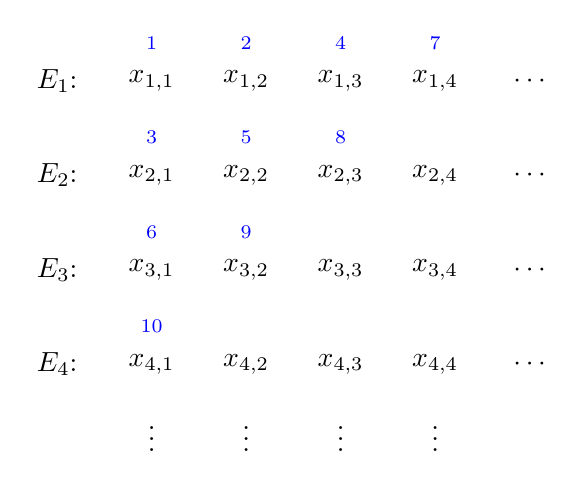
\begin{tikzpicture}[scale=1.2]
    % Grid elements with enumeration order
    \node at (0,3) {$x_{1,1}$};
    \node[blue, font=\scriptsize] at (0,3.4) {1};
    \node at (1,3) {$x_{1,2}$};
    \node[blue, font=\scriptsize] at (1,3.4) {2};
    \node at (2,3) {$x_{1,3}$};
    \node[blue, font=\scriptsize] at (2,3.4) {4};
    \node at (3,3) {$x_{1,4}$};
    \node[blue, font=\scriptsize] at (3,3.4) {7};
    \node at (4,3) {$\cdots$};

    \node at (0,2) {$x_{2,1}$};
    \node[blue, font=\scriptsize] at (0,2.4) {3};
    \node at (1,2) {$x_{2,2}$};
    \node[blue, font=\scriptsize] at (1,2.4) {5};
    \node at (2,2) {$x_{2,3}$};
    \node[blue, font=\scriptsize] at (2,2.4) {8};
    \node at (3,2) {$x_{2,4}$};
    \node at (4,2) {$\cdots$};

    \node at (0,1) {$x_{3,1}$};
    \node[blue, font=\scriptsize] at (0,1.4) {6};
    \node at (1,1) {$x_{3,2}$};
    \node[blue, font=\scriptsize] at (1,1.4) {9};
    \node at (2,1) {$x_{3,3}$};
    \node at (3,1) {$x_{3,4}$};
    \node at (4,1) {$\cdots$};

    \node at (0,0) {$x_{4,1}$};
    \node[blue, font=\scriptsize] at (0,0.4) {10};
    \node at (1,0) {$x_{4,2}$};
    \node at (2,0) {$x_{4,3}$};
    \node at (3,0) {$x_{4,4}$};
    \node at (4,0) {$\cdots$};

    \node at (0,-0.7) {$\vdots$};
    \node at (1,-0.7) {$\vdots$};
    \node at (2,-0.7) {$\vdots$};
    \node at (3,-0.7) {$\vdots$};

    % Row labels
    \node at (-1,3) {$E_1$:};
    \node at (-1,2) {$E_2$:};
    \node at (-1,1) {$E_3$:};
    \node at (-1,0) {$E_4$:};
\end{tikzpicture}
\end{center}

We enumerate the union by traversing diagonals: first $x_{1,1}$, then $x_{1,2}, x_{2,1}$, then $x_{1,3}, x_{2,2}, x_{3,1}$, and so on. The $k$-th diagonal contains all $x_{n,m}$ with $n + m = k + 1$.

This gives a surjection from $\N$ onto $\bigcup_{n=1}^{\infty} E_n$ (skipping repeats if sets overlap). Thus the union is countable.
\end{proof}

\begin{notebox}
\textbf{Note:} The \defn{diagonal argument} is a powerful technique for enumerating countable unions. By arranging elements in a grid and traversing along diagonals, we reduce a ``two-dimensional'' infinite collection to a ``one-dimensional'' sequence.
\end{notebox}


\begin{theorem}
If $A$ is countable, then $A^n$ is countable for all $n \in \N$.
\end{theorem}

\begin{proof}
By induction on $n$.

\textbf{Base case ($n = 1$):} $A^1 = A$ is countable by assumption.

\textbf{Inductive hypothesis:} Assume $A^n$ is countable for some $n \geq 1$.

\textbf{Inductive step:} We show $A^{n+1}$ is countable. Observe that
\[
A^{n+1} = A^n \times A.
\]
By the inductive hypothesis, $A^n$ is countable, so we can enumerate it as $A^n = \{b_1, b_2, b_3, \ldots\}$. Since $A$ is countable by assumption, we can write $A = \{a_1, a_2, a_3, \ldots\}$. The Cartesian product $A^n \times A$ can then be arranged in a grid:
\[
\begin{array}{cccc}
(b_1, a_1) & (b_1, a_2) & (b_1, a_3) & \cdots \\
(b_2, a_1) & (b_2, a_2) & (b_2, a_3) & \cdots \\
(b_3, a_1) & (b_3, a_2) & (b_3, a_3) & \cdots \\
\vdots & \vdots & \vdots & \ddots
\end{array}
\]
By the diagonal argument, $A^n \times A$ is countable.

\textbf{Conclusion:} By the principle of mathematical induction, $A^n$ is countable for all $n \in \N$.
\end{proof}

\begin{corollary}
$\Q$ is countable.
\end{corollary}

\begin{proof}
For each $n \in \N$, let $E_n = \left\{\frac{m}{n} : m \in \Z\right\}$ be the set of rationals with denominator $n$. Each $E_n$ is countable (since $E_n \sim \Z$ and $\Z$ is countable). Then
\[
\Q = \bigcup_{n=1}^{\infty} E_n
\]
is a countable union of countable sets, hence countable.
\end{proof}

\begin{theorem}[$\R$ is uncountable]
The set of binary sequences $\{0,1\}^{\N}$ is uncountable.
\end{theorem}

\begin{proof}
By contradiction. Suppose $\{0,1\}^{\N}$ is countable. Then we can list all binary sequences as $s_1, s_2, s_3, \ldots$ where each $s_n = (s_{n,1}, s_{n,2}, s_{n,3}, \ldots)$:

\begin{center}
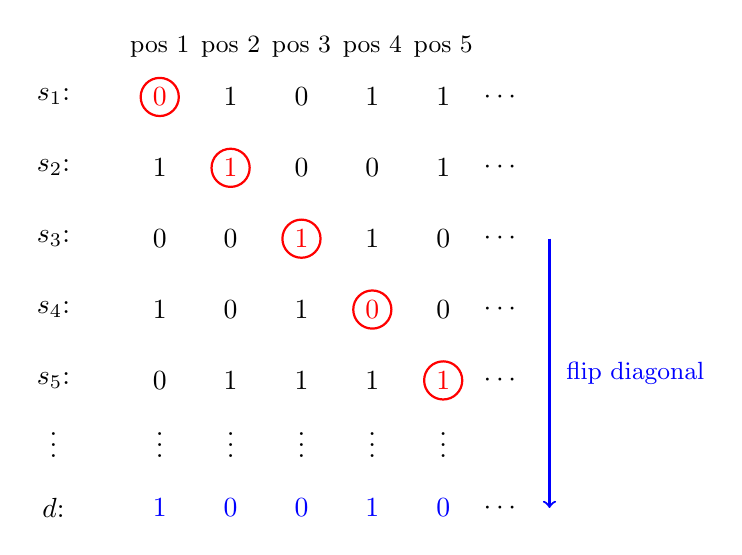
\begin{tikzpicture}[scale=0.9]
    % Column headers
    \node at (1.5,4.2) {\small pos 1};
    \node at (2.5,4.2) {\small pos 2};
    \node at (3.5,4.2) {\small pos 3};
    \node at (4.5,4.2) {\small pos 4};
    \node at (5.5,4.2) {\small pos 5};

    % Row labels
    \node at (0,3.5) {$s_1$:};
    \node at (0,2.5) {$s_2$:};
    \node at (0,1.5) {$s_3$:};
    \node at (0,0.5) {$s_4$:};
    \node at (0,-0.5) {$s_5$:};

    % Grid entries - row 1
    \node[draw, circle, thick, red, inner sep=2pt] at (1.5,3.5) {$0$};
    \node at (2.5,3.5) {$1$};
    \node at (3.5,3.5) {$0$};
    \node at (4.5,3.5) {$1$};
    \node at (5.5,3.5) {$1$};
    \node at (6.3,3.5) {$\cdots$};

    % Grid entries - row 2
    \node at (1.5,2.5) {$1$};
    \node[draw, circle, thick, red, inner sep=2pt] at (2.5,2.5) {$1$};
    \node at (3.5,2.5) {$0$};
    \node at (4.5,2.5) {$0$};
    \node at (5.5,2.5) {$1$};
    \node at (6.3,2.5) {$\cdots$};

    % Grid entries - row 3
    \node at (1.5,1.5) {$0$};
    \node at (2.5,1.5) {$0$};
    \node[draw, circle, thick, red, inner sep=2pt] at (3.5,1.5) {$1$};
    \node at (4.5,1.5) {$1$};
    \node at (5.5,1.5) {$0$};
    \node at (6.3,1.5) {$\cdots$};

    % Grid entries - row 4
    \node at (1.5,0.5) {$1$};
    \node at (2.5,0.5) {$0$};
    \node at (3.5,0.5) {$1$};
    \node[draw, circle, thick, red, inner sep=2pt] at (4.5,0.5) {$0$};
    \node at (5.5,0.5) {$0$};
    \node at (6.3,0.5) {$\cdots$};

    % Grid entries - row 5
    \node at (1.5,-0.5) {$0$};
    \node at (2.5,-0.5) {$1$};
    \node at (3.5,-0.5) {$1$};
    \node at (4.5,-0.5) {$1$};
    \node[draw, circle, thick, red, inner sep=2pt] at (5.5,-0.5) {$1$};
    \node at (6.3,-0.5) {$\cdots$};

    % Vdots
    \node at (0,-1.3) {$\vdots$};
    \node at (1.5,-1.3) {$\vdots$};
    \node at (2.5,-1.3) {$\vdots$};
    \node at (3.5,-1.3) {$\vdots$};
    \node at (4.5,-1.3) {$\vdots$};
    \node at (5.5,-1.3) {$\vdots$};

    % The new sequence
    \node at (0,-2.3) {$d$:};
    \node[blue, font=\bfseries] at (1.5,-2.3) {$1$};
    \node[blue, font=\bfseries] at (2.5,-2.3) {$0$};
    \node[blue, font=\bfseries] at (3.5,-2.3) {$0$};
    \node[blue, font=\bfseries] at (4.5,-2.3) {$1$};
    \node[blue, font=\bfseries] at (5.5,-2.3) {$0$};
    \node at (6.3,-2.3) {$\cdots$};

    % Arrow and label
    \draw[->, thick, blue] (7,1.5) -- (7,-2.3);
    \node[right, blue] at (7.1,-0.4) {\small flip diagonal};
\end{tikzpicture}
\end{center}

Construct a new sequence $d = (d_1, d_2, d_3, \ldots)$ by flipping the diagonal entries:
\[
d_n = \begin{cases} 1 & \text{if } s_{n,n} = 0 \\ 0 & \text{if } s_{n,n} = 1 \end{cases}
\]

Then $d$ differs from $s_n$ in the $n$-th position for every $n \in \N$. Thus $d \neq s_n$ for all $n$, so $d$ is not in our list. But $d \in \{0,1\}^{\N}$, contradicting that our list contains all binary sequences.

Therefore $\{0,1\}^{\N}$ is uncountable.
\end{proof}

\begin{notebox}
\textbf{Note:} This is \defn{Cantor's diagonal argument}. Since there is a bijection between $\{0,1\}^{\N}$ and $\R$ (via binary expansions), this proves $\R$ is uncountable. The key insight is that any proposed enumeration can be ``diagonalized'' to produce a missing element.
\end{notebox}

\textbf{Exercise:} An \defn{algebraic number} is a solution to a polynomial equation with coefficients in $\Q$:
\[
a_n x^n + a_{n-1} x^{n-1} + \cdots + a_1 x + a_0 = 0, \quad a_i \in \Q.
\]
Is the set of algebraic numbers countable?

\textit{Proof:} Yes. We proceed by induction on the degree of the polynomial.

\textbf{Base case ($n = 1$):} A degree-1 polynomial $mx + b = 0$ has solution $x = -b/m \in \Q$. Since $\Q$ is countable, the set of algebraic numbers of degree 1 is countable.

\textbf{Inductive step:} Let $A_n$ denote the set of algebraic numbers that are roots of some polynomial of degree at most $n$. Assume $A_n$ is countable. Consider numbers of the form
\[
\{a + b \cdot \sqrt[n+1]{z} : a, b, z \in A_n\}.
\]
This set is countable since $A_n^3$ is countable (as a finite Cartesian product of a countable set). More generally, the set of polynomials of degree $n+1$ with coefficients in $\Q$ is $\Q^{n+2}$, which is countable. Each such polynomial has at most $n+1$ roots, so the roots form a countable union of finite sets, hence $A_{n+1}$ is countable.

\textbf{Conclusion:} The set of all algebraic numbers is $\bigcup_{n=1}^{\infty} A_n$, a countable union of countable sets, hence countable.

\begin{notebox}
\textbf{Note:} A real number that is \emph{not} algebraic is called \defn{transcendental}. Since the algebraic numbers are countable but $\R$ is uncountable, transcendental numbers must exist---in fact, ``most'' real numbers are transcendental! Examples include $\pi$, $e$, and $\tau = 2\pi$. Proving that a specific number is transcendental is typically very difficult: Lindemann proved $\pi$ is transcendental in 1882, and Hermite proved $e$ is transcendental in 1873.
\end{notebox}

\begin{remark}
Recall the \textbf{Cantor set} from Lecture 2: the set of all points in $[0,1]$ whose ternary expansion uses only the digits $0$ and $2$. The Cantor set is in bijection with $\{0,2\}^{\N} \sim \{0,1\}^{\N}$ (just map $0 \mapsto 0$ and $2 \mapsto 1$). By the same diagonal argument, the Cantor set is uncountable---despite being ``sparse'' (it contains no intervals and has measure zero).
\end{remark}

\end{document}
